\documentclass{article}
\usepackage{ctex}

% Set page size and margins
% Replace `letterpaper' with `a4paper' for UK/EU standard size
\usepackage[letterpaper,top=2cm,bottom=2cm,left=2.5cm,right=2.5cm,marginparwidth=1.75cm]{geometry}

% Useful packages
\usepackage{amsmath}
\usepackage{graphicx}
\usepackage{subfigure}
\usepackage{float}
\usepackage[colorlinks=true, allcolors=blue]{hyperref}

\title{微分方程数值解计算实习课后作业8}
\author{陈文宇}
\date{\today}


\begin{document}


\maketitle

\tableofcontents

\newpage
%---------------------------------------------------
\section{问题重述}

\begin{itemize}
    \item 画出数值解的图像
    \item 获取两类误差:
    $$ errL=(\int_{\Omega}(\mu_{h}(x)-\mu(x))^{2}dxdy)^{\frac{1}{2}}$$
    $$ errH=(\int_{\Omega}(\mu_{h}(x)-\mu(x))^{2}+(\partial_{x}\mu_{h}(x)-\partial_{x}\mu(x))^{2}+(\partial_{y}\mu_{h}(x)-\partial_{y}\mu(x))^{2}dxdy)^{\frac{1}{2}}$$
    计算其关于网格长度的数值收敛阶
    \item 用$loglog()$函数展示$errL2,errH1,condA$的图像,
\end{itemize}
 
%---------------------------------------------------
\section{实验思路}
二维三角Lagrange型有限元方法求解练习:
\[
\left\{
\begin{aligned}
	&-\mu '' + \frac{\pi^{2}}{4}\mu = \frac{\pi^{2}}{2}\sin{\frac{\pi}{2}x} \quad0<x<1 
	\\
	&\mu(0,y)=0 ,\quad \mu(x,1)=0 
        \\
        &\partial_{x}\mu(1,y)=y-\pi\cos(\pi x)\sin(\pi y) \quad (1,y)\in\partial\Omega
        \\
        &\partial_{y}\mu(x,1)=x-\pi\sin(\pi x)\cos(\pi y) \quad (x,1)\in\partial\Omega
\end{aligned}
\right.
\]

确定单元刚度矩阵脚标和刚度矩阵脚标的对应关系后,形成有限元方程后,对其本质边界条件做处理(此处对于左边界和下边界的处理是简单的,对于右边界和上边界的处理可以在右端向量中完成),刚度矩阵是大型稀疏矩阵,可以通过sparse函数将其转化为稀疏矩阵的存储形式,求解线性方程组$Ax=b$即可获得基函数系数。
对于条件数可以使用matlab命令$condest(A)$,
定义errL和errH后,给出其在相应区间的函数值,然后可以使用三角元的Gauss四点求积公式来求积分,
进而使用$loglog$函数绘制图像即可。

matlab编程的具体操作详见FEM\_2D1PDelta\_L.m,在代码结构上采用了实习课老师分享的代码。
对于刚度矩阵,代码中仍旧先生成单元刚度矩阵,再扩建为整个刚度矩阵。


\newpage
%---------------------------------------------------
\section{实验结果}

下图是数值解和精确解的图像:
\begin{figure}[H]
\subfigure[正视图]{
\begin{minipage}[t]{0.32\linewidth}
\centering
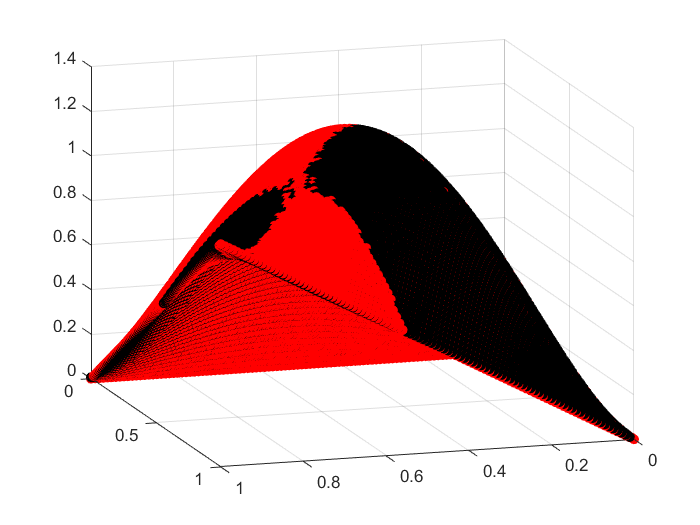
\includegraphics[scale=0.3]{solution_image1.png}
\end{minipage}
}
\subfigure[侧视图]{
\begin{minipage}[t]{0.32\linewidth}
\centering
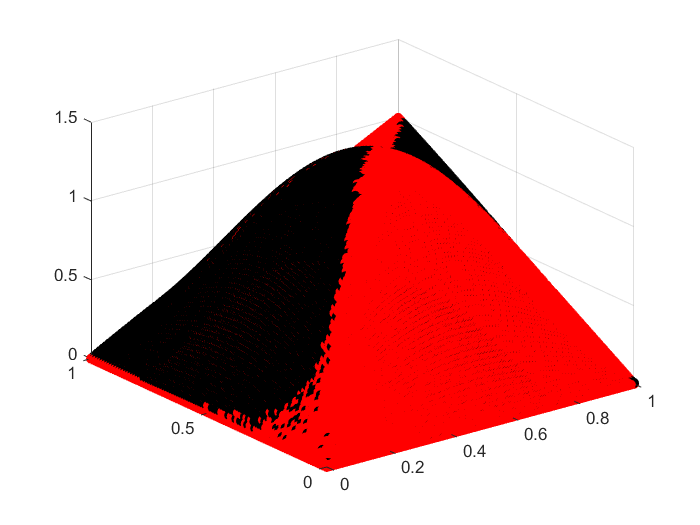
\includegraphics[scale=0.3]{solution_image2.png}
\end{minipage}
}
\subfigure[后视图]{
\begin{minipage}[t]{0.32\linewidth}
\centering
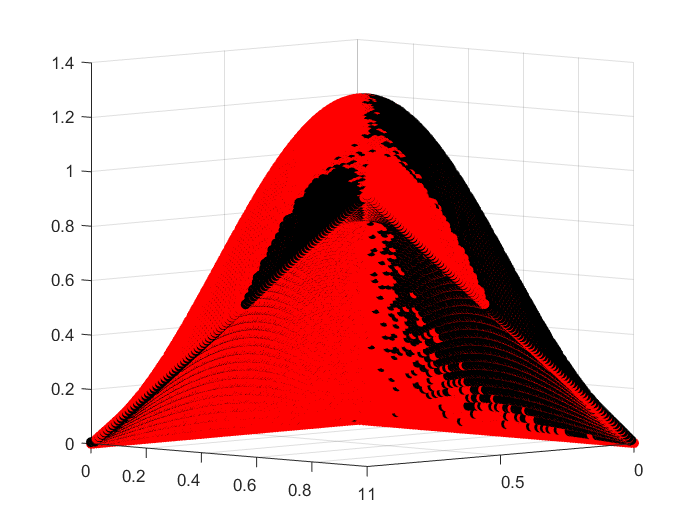
\includegraphics[scale=0.3]{solution_image3.png}
\end{minipage}
}

\caption{\label{solution_image}数值解和精确解的图像}

\end{figure}

下图是$(logh,log(errL))$的图像,同$y=h^2$对比知,$errL$收敛阶为2.
\begin{figure}[H]
\centering
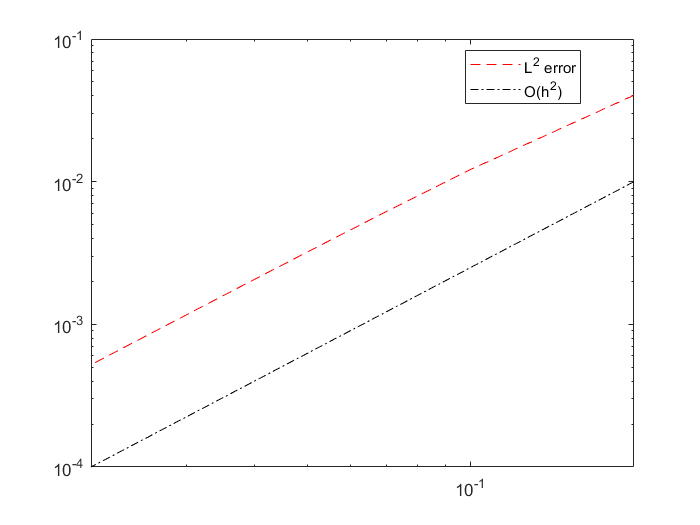
\includegraphics[scale=0.5]{errL2.png}
\caption{\label{L_err}$L^{2}([0,1])$误差的收敛阶}
\end{figure}

\newpage
下图是$(logh,log(errH))$的图像,根据线性基本拟合,知$errH$收敛阶为1.
\begin{figure}[H]
\centering
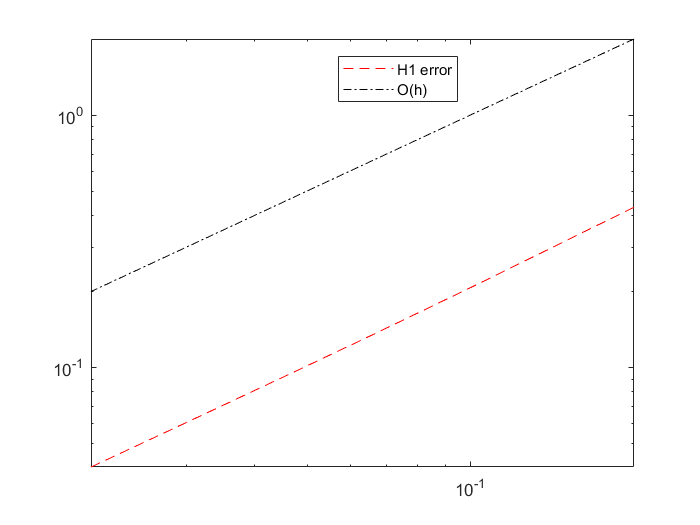
\includegraphics[scale=0.5]{errH1.png}
\caption{\label{H1_err}$H^{1}([0,1])$误差的收敛阶}
\end{figure}



用$loglog()$函数展示矩阵A的条件数的变化。
\begin{figure}[H]
\centering
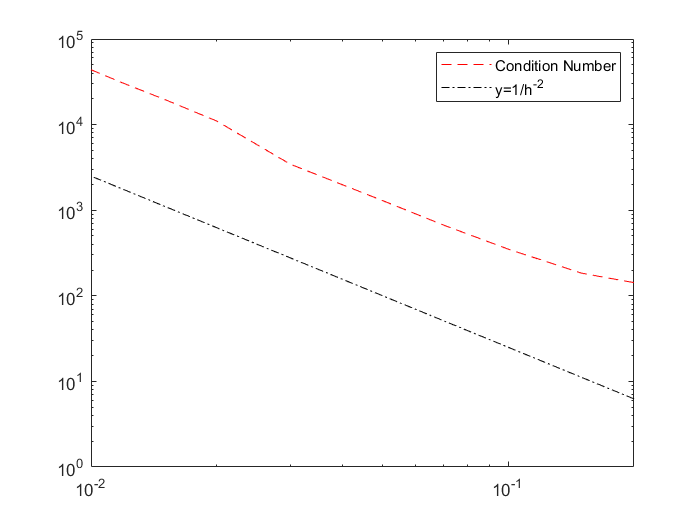
\includegraphics[scale=0.5]{CondA.png}
\caption{\label{CondA}$CondA$}
\end{figure}


%-----------------------------------------------------
\section{实验结果分析}
对于本题,L2误差的收敛阶为2,H1误差的和收敛阶为1,矩阵A条件数$CondA$与同$h$成指数关系,且与$h^{-2}$同阶。
\end{document}